\documentclass[a4paper,10pt,twocolumn]{scrartcl}
\pagestyle{plain}
\usepackage[left=2cm,right=2cm,top=2.5cm,bottom=2.5cm]{geometry}

\usepackage[utf8]{inputenc}
\usepackage[T1]{fontenc}
\usepackage{hyphenat}
\usepackage{lipsum}
\usepackage{graphicx}
\usepackage{caption}
\usepackage{hyperref}
\hypersetup{
	colorlinks=true,
	linkcolor=blue,     
	urlcolor=blue,
}


\author{Frank Ebel 01429282, Josef Glas 08606876\\Felix Korbelius 01526132, Johannes Schabbauer 11776224}
\title{\vspace*{-1cm}Management Summary DOPP Exercise 3}
\subtitle{Group 10, Question 20}
\date{\today \vspace*{-0.8cm}}




\begin{document}
\sffamily
\maketitle

This is the Management Summary of the third exercise, lecture \emph{Data-oriented Programming Paradigms} (188.995) for the question 20 from the task. The work was done equally by all collaborators of group 20 mentioned above. The aim of this document is to present the task, the approach and the findings of the investigations in a way as easy to follow as possible.

\section{Questions}

\section{Approach}

\section{Findings}

\begin{figure}[h]
	\centering
 	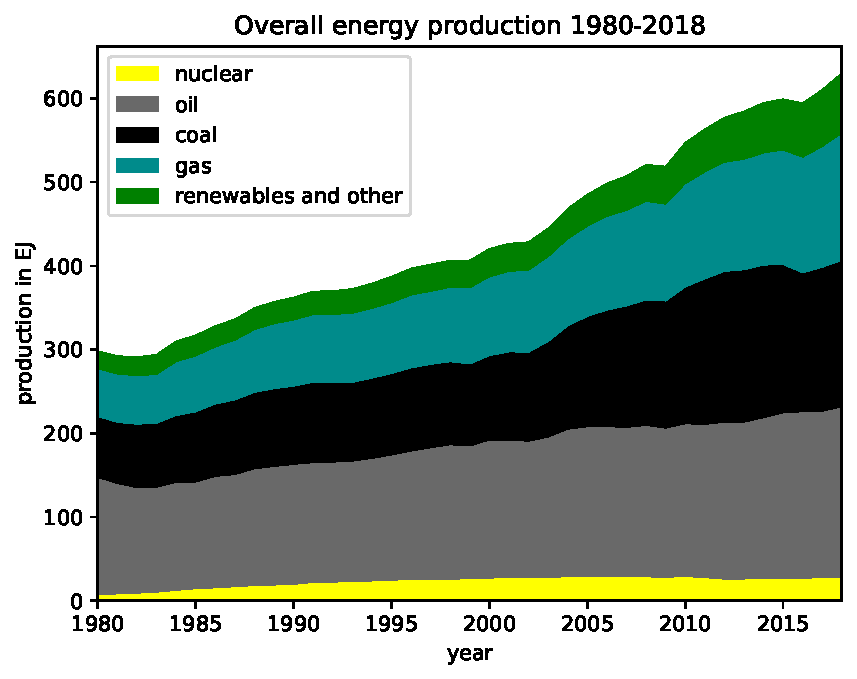
\includegraphics[width=\columnwidth]{../figures/q1_plot1.pdf}
 	\captionof{figure}{Constitution of worldwide energy production over time.}
 	\label{fig:q1_plot1}
\end{figure}

\begin{figure*}[hbt]
	\centering
	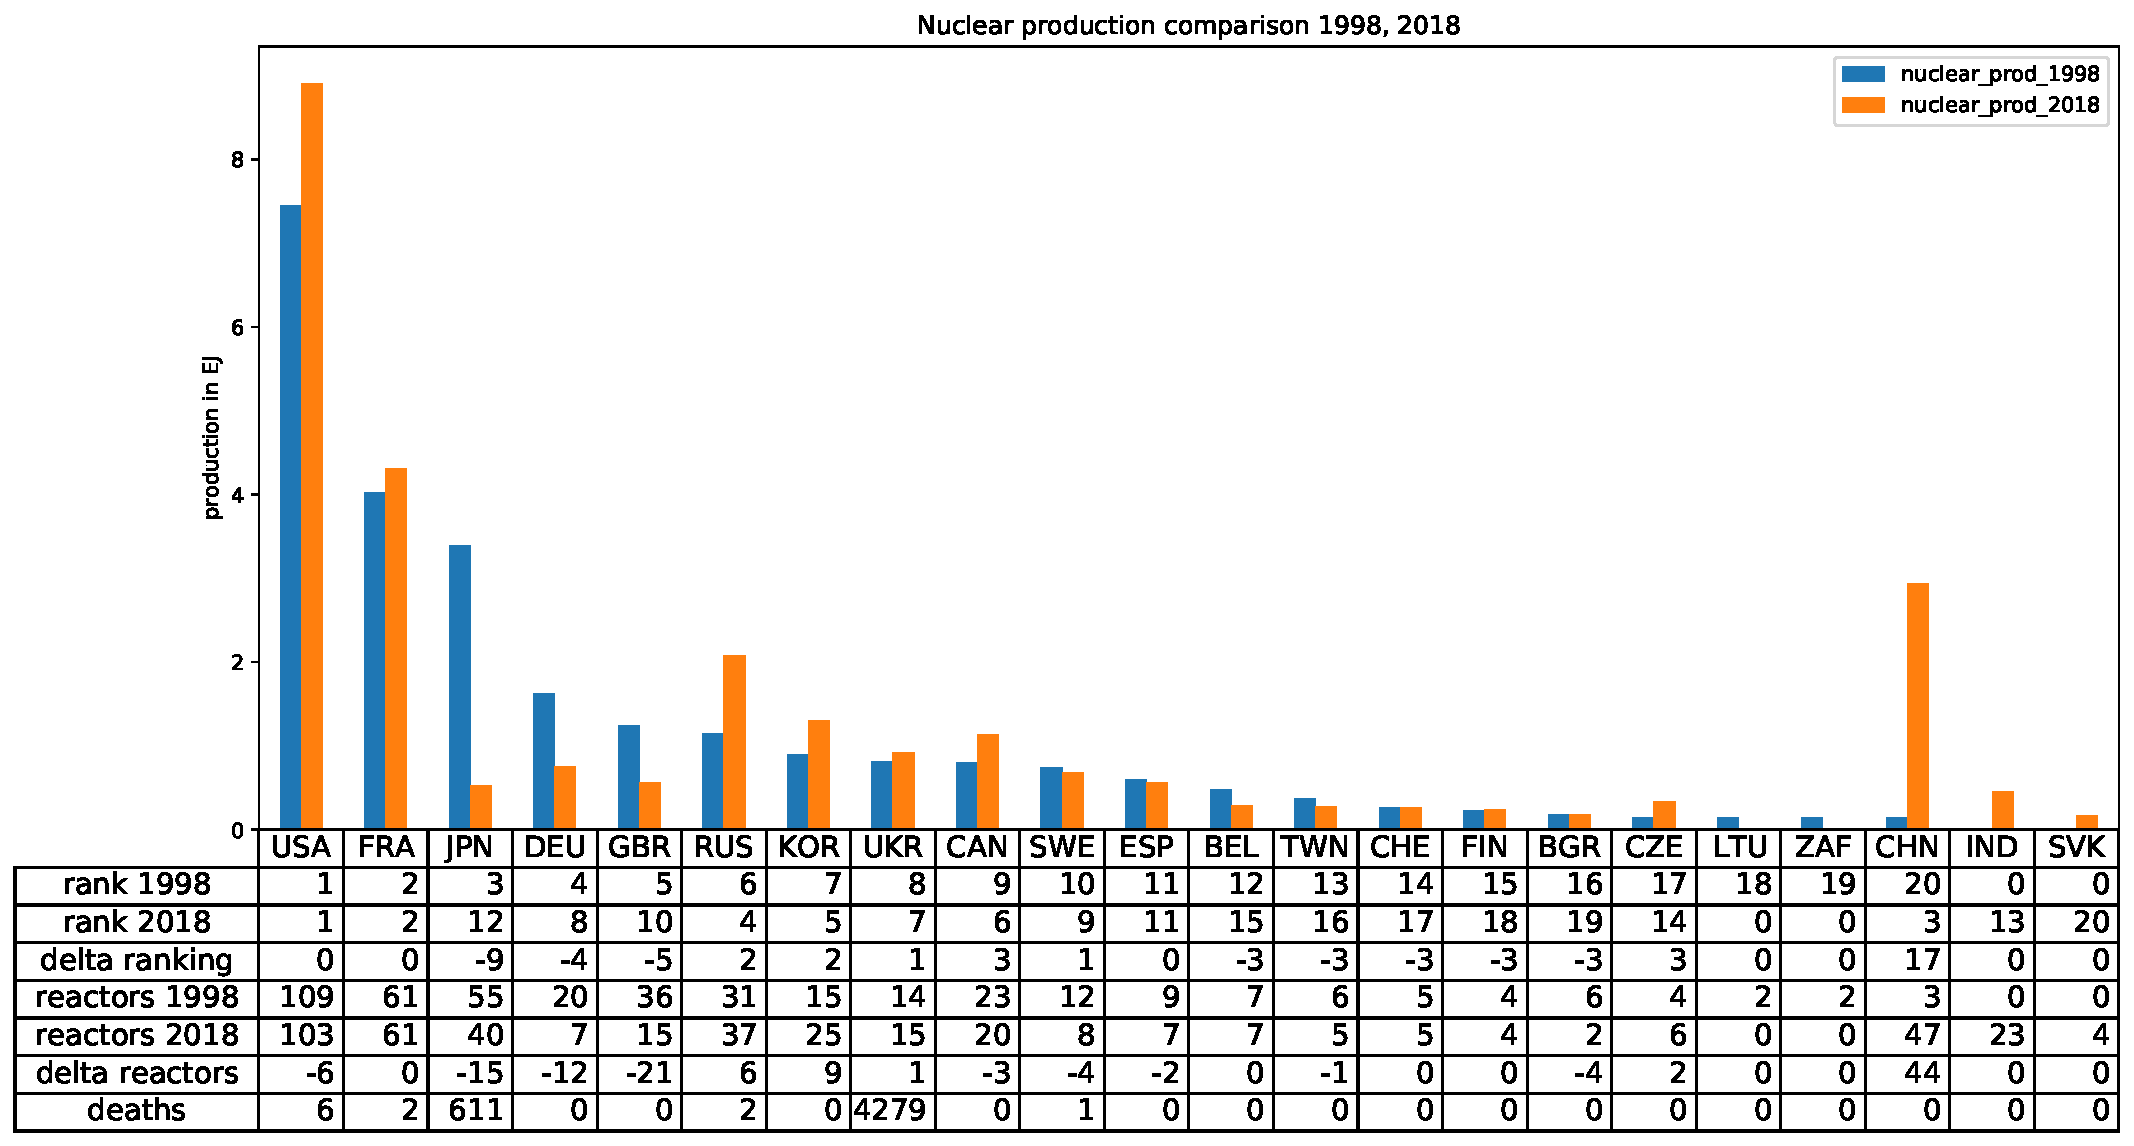
\includegraphics[width=\textwidth]{../figures/q1_plot2.pdf}
	\caption{Largest producers of nuclear energy in 2018, compared to their produced nuclear energy in 1998.}
	\label{fig:q2_plot2}
\end{figure*}

\lipsum{1}
\end{document}
